Niniejszy podrozdział przedstawia różne badania, których celem jest ewaluacja klasyfikacji YOLOv8n na przykładzie klasy człowiek. Model zbadano pod kątem wpływu jak manipulacja poziomem oświetlenia oraz progu ufności przekłada się na jego wyniki. Dla każdego zmierzonego progu ufności wyznaczane będą metryki potrzebne do zobrazowania wniosków. Będą one liczone na podstawie poprzednio uzyskanych metryk --- TP, TN, FP i FN. Do testu wykrzystano cztery filmy. Każdy z nich przedstawia wyłącznie człowieka. Wartości jasności i nasycenia przedstawiono w tabeli \ref{tab:saturacja-jasnosc-czlowiek}. Wygląd nagranego pomieszczenia dla różnych poziomów oświetlenia ukazano na rysunku \ref{fig:person_grid}. 

\begin{table}[H]
\centering
\caption{Jasność i nasycenie dla wszystkich filmów.}
\begin{tabular}{|c|c|c|c|}
\hline
Poziom oświetlenia  & Obecne obiekty & Jasność & Nasycenie \\ \hline
1        & człowiek       & 152.73  & 107.3     \\ \hline
2        & człowiek       & 134.64  & 93.48     \\ \hline
3        & człowiek       & 41.59   & 123.48    \\ \hline
4        & człowiek       & 25.47   & 90.92     \\ \hline
\end{tabular}

\label{tab:saturacja-jasnosc-czlowiek}
\end{table}


\subsection{Ewaluacja modelu dla różnych poziomów oświetlenia}
\label{sec:test-AUC}
W celu zobrazowania i oceniania wyniku modelu zastosowano metrykę 

\begin{figure}[H]
    \centering
    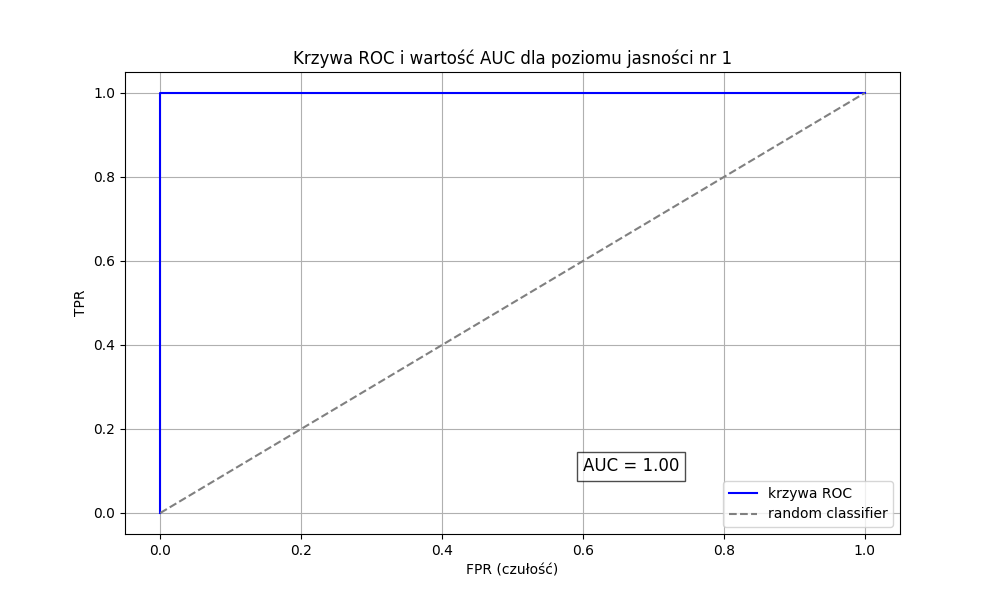
\includegraphics[width=\linewidth]{r_test_dokładności/AUC_charts/1.png}
    \caption{Krzywa ROC i wartość AUC dla poziomu jasności nr 1.}
    \label{fig:ROC-1}
\end{figure}

\begin{figure}[H]
    \centering
    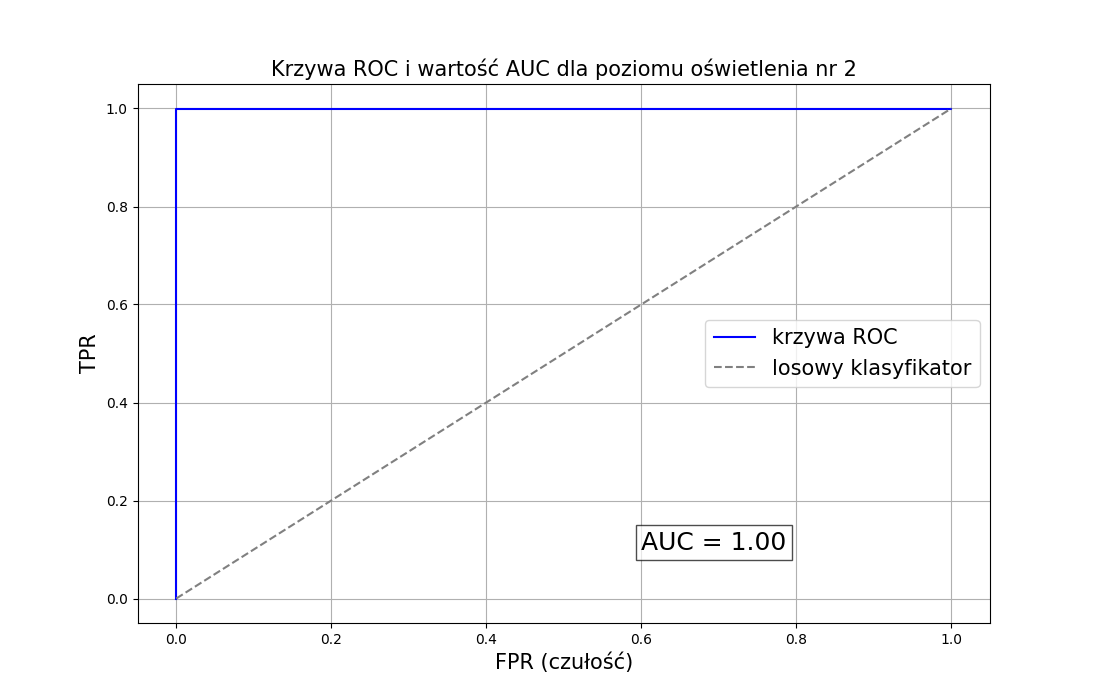
\includegraphics[width=\linewidth]{r_test_dokładności/AUC_charts/2.png}
    \caption{Krzywa ROC i wartość AUC dla poziomu jasności nr 2.}
    \label{fig:ROC-2}
\end{figure}

\begin{figure}[H]
    \centering
    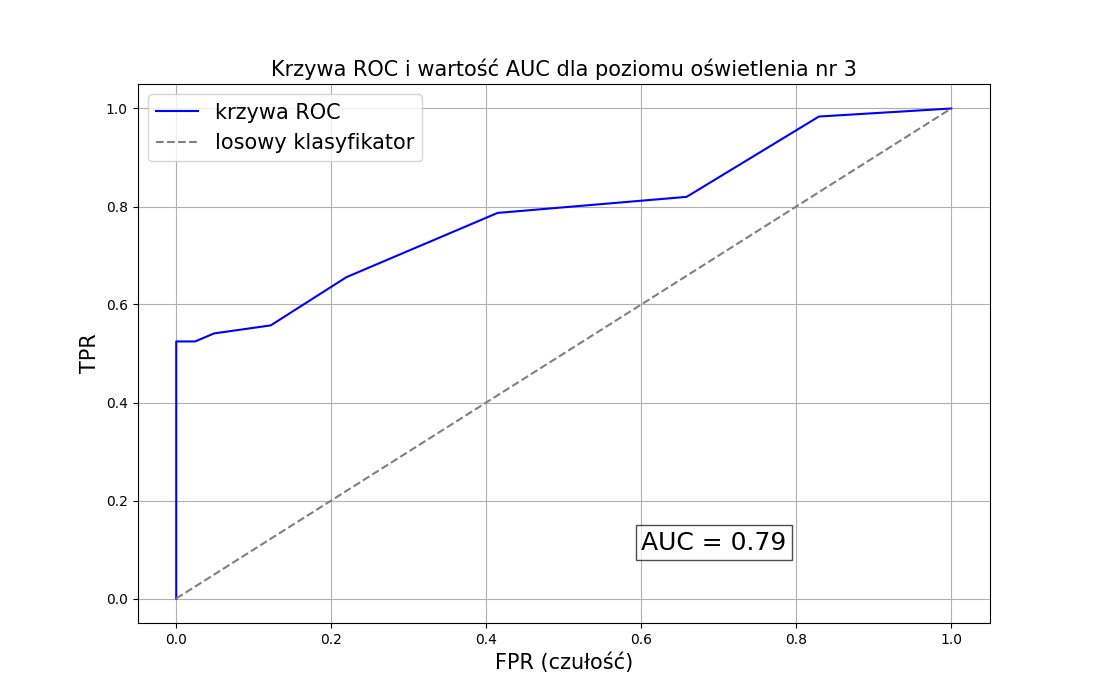
\includegraphics[width=\linewidth]{r_test_dokładności/AUC_charts/3.png}
    \caption{Krzywa ROC i wartość AUC dla poziomu jasności nr 3.}
    \label{fig:ROC-3}
\end{figure}

\begin{figure}[H]
    \centering
    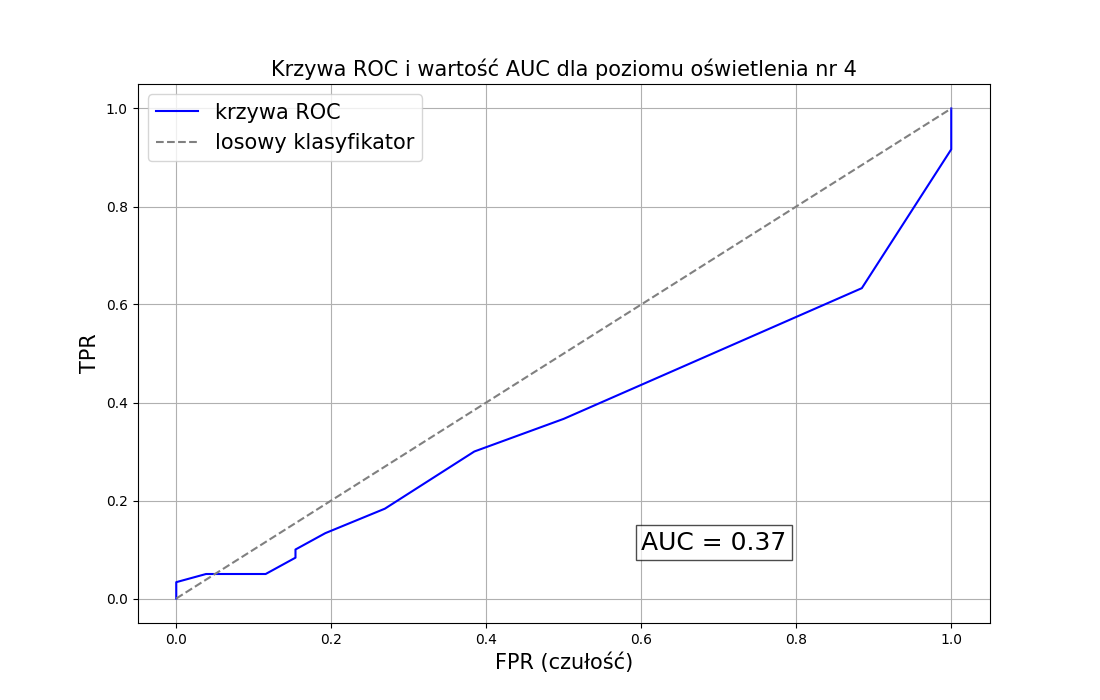
\includegraphics[width=\linewidth]{r_test_dokładności/AUC_charts/4.png}
    \caption{Krzywa ROC i wartość AUC dla poziomu jasności nr 4.}
    \label{fig:ROC-4}
\end{figure}

\begin{figure}[H]
    \centering
    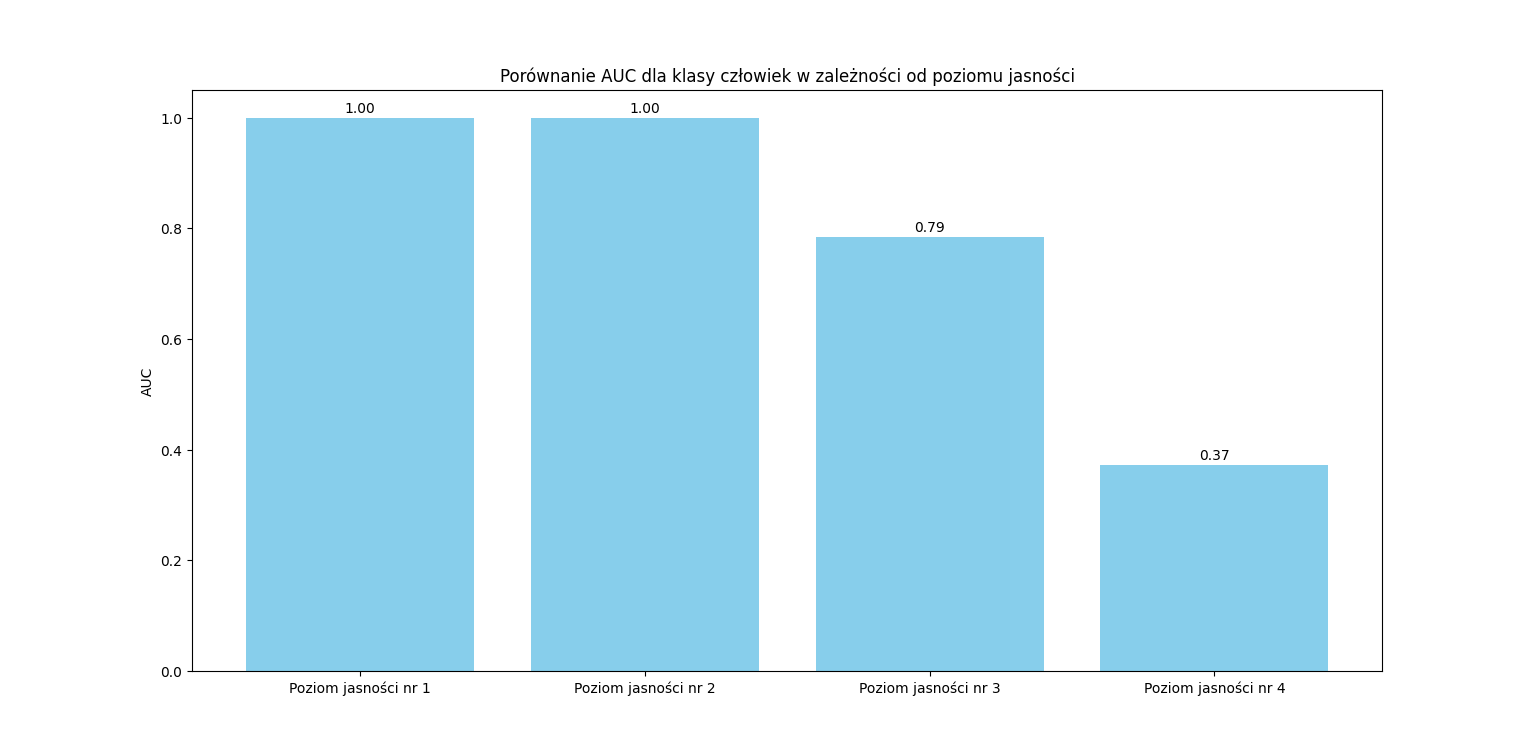
\includegraphics[width=\linewidth]{r_test_dokładności/AUC_charts/porownanieAUC.png}
    \caption{Wykres porównujący wartości AUC dla zbadanych poziomów jasności.}
    \label{fig:AUC}
\end{figure}



\subsection{Analiza wpływu progu ufności na wyniki detekcji}

